\documentclass[technologies,article,submit,pdftex,moreauthors]{Definitions/mdpi}

\usepackage{adjustbox}
\usepackage{placeins}
\usepackage{tikz}
\usetikzlibrary{arrows.meta,positioning,shapes.geometric}

\firstpage{1}
\makeatletter
\setcounter{page}{\@firstpage}
\makeatother
\pubvolume{1}
\issuenum{1}
\articlenumber{0}
\pubyear{2026}
\copyrightyear{2026}
\datereceived{}
\daterevised{}
\dateaccepted{}
\datepublished{}

\Title{Supplementary Material: Experimental Characterization of a Low-Cost IoT Electrical Monitoring System for Traceable Machine-Level Energy Performance Indicators}
\Author{Andrés Viveros $^{1}$, Ivan Derpich $^{1,}$*, Juan Miguel Sepulveda $^{1}$, and Armando Meza $^{1}$}
\AuthorNames{Andrés Viveros, Ivan Derpich, Juan Miguel Sepulveda and Armando Meza}
\address{$^{1}$ \quad Centre for Innovation in Technology and Design of Materials for the Built Environment (CIMAC), ANID CTI250005, and Department of Industrial Engineering, Faculty of Engineering, Universidad de Santiago de Chile, Santiago, Chile}
\corres{Correspondence: ivan.derpich@usach.cl}
\abstract{Supplementary tables and figures supporting the literature positioning, architecture description, reproducibility information, experimental characterization, and bounded industrial demonstration reported in the main manuscript.}
\keyword{industrial sensors; electrical sensing; IoT metering; energy performance indicator; supplementary material}

\renewcommand{\thetable}{S\arabic{table}}
\renewcommand{\thefigure}{S\arabic{figure}}

\begin{document}

\section{Supplementary Literature and Architecture Details}
This Supplementary Material provides supporting tables and figures that complement the main manuscript. It includes the extended gap synthesis, functional-layer summary, platform screenshots, reproducibility details, segment-preserving bootstrap results, firmware continuity logic, PCB bill of materials, and additional scenario visualizations.

\begin{table}[H]
\caption{Supplementary critical synthesis of related literature and the gap addressed by EnPi.}
\label{tab:S1}
\centering
\scriptsize
\begin{adjustbox}{max width=\columnwidth}
\begin{tabular}{p{0.30\columnwidth}p{0.17\columnwidth}p{0.48\columnwidth}}
\toprule
Line & Refs. & Gap with respect to EnPi \\
\midrule
Smart energy management IoT & [1], [4] & Does not centrally integrate progressive adoption, production, or EnPI traceability. \\
Industrial Energy Management Systems & [2], [3] & Assumes greater digital maturity and instrumentation than many industrial SMEs have. \\
Web and IIoT platforms & [5], [10], [14], [15] & Provides interoperability and digital services, but is not centered on equipment-level energy metering or EnPI reporting. \\
Smart grids, privacy, and sustainable IoT & [6]-[9], [11] & Addresses transversal requirements, not an incremental energy-adoption architecture. \\
Systems engineering and energy-IoT architectures & \cite{ref26,ref27,ref28} & Frames integration, interoperability, and system management challenges, but does not directly operationalize EnPI traceability for industrial SMEs. \\
NILM and load monitoring & [21] & Introduces disaggregation uncertainty; EnPi prioritizes direct metering at selected points. \\
Energy standards and indicators & [19], [20] & Requires traceable data connected to operation; EnPi seeks to cover this operational bridge. \\
Energy benchmark and IoT monitor validation & [22]--[24] & Provides comparison ranges or low-cost validation examples, but does not by itself articulate SaaS traceability, production, and equipment-level EnPI. \\
\bottomrule
\end{tabular}
\end{adjustbox}
\end{table}

\begin{table}[!htbp]
\caption{Supplementary functional layers of the EnPi architecture.}
\label{tab:S2}
\centering
\scriptsize
\begin{adjustbox}{max width=\textwidth}
\begin{tabular}{p{0.1\textwidth}p{0.35\textwidth}p{0.35\textwidth}}
\toprule
Layer & Function & Expected outcome \\
\midrule
Acquisition & Manual upload of bills, historical records, existing meters, and IoT nodes. & Energy data captured from available sources and new measurements. \\
Integration & Normalization by company, facility, work center, machine, meter, and period. & Common model for comparing consumption and assigning responsibility. \\
SaaS & Management of users, roles, catalogs, dashboards, reports, and assets. & Centralized web access for operation, analysis, and decision-making. \\
Analytics & EnPI indicators, baselines, trends, deviations, thresholds, and alert rules. & Actionable information on energy per unit produced, process, or period. \\
Governance & Traceability of origin, responsible party, period, capture method, privacy, and data reconciliation. & Greater confidence for internal use, audit, and reporting. \\
Decision & Prioritization of improvements, follow-up of measures, evidence, and technological scaling. & Preparation of traceable evidence and continuous improvement. \\
\bottomrule
\end{tabular}
\end{adjustbox}
\end{table}


\FloatBarrier


\section{Supplementary Platform and Traceability Views}

\begin{figure}[H]
\centering
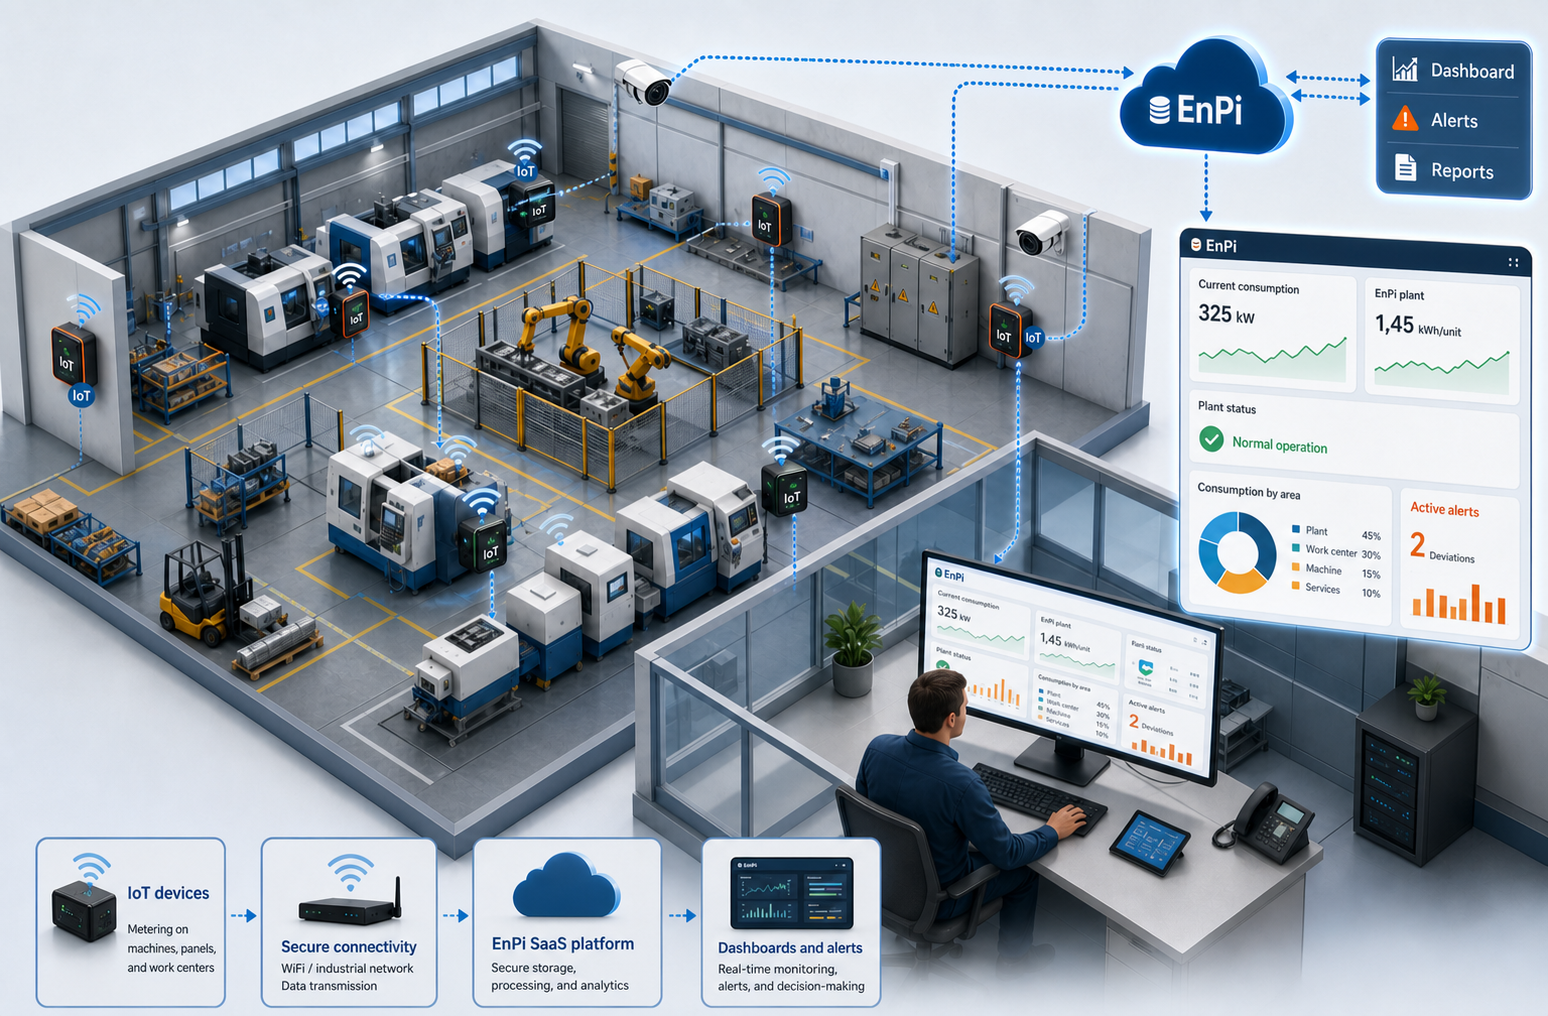
\includegraphics[width=0.92\textwidth]{figures/image2.png}
\caption{Supplementary conceptual progressive deployment scenario through intelligent energy-metering nodes and contextual support cameras for alerts.}
\label{fig:S1}
\end{figure}


\begin{figure}[!htbp]
\centering
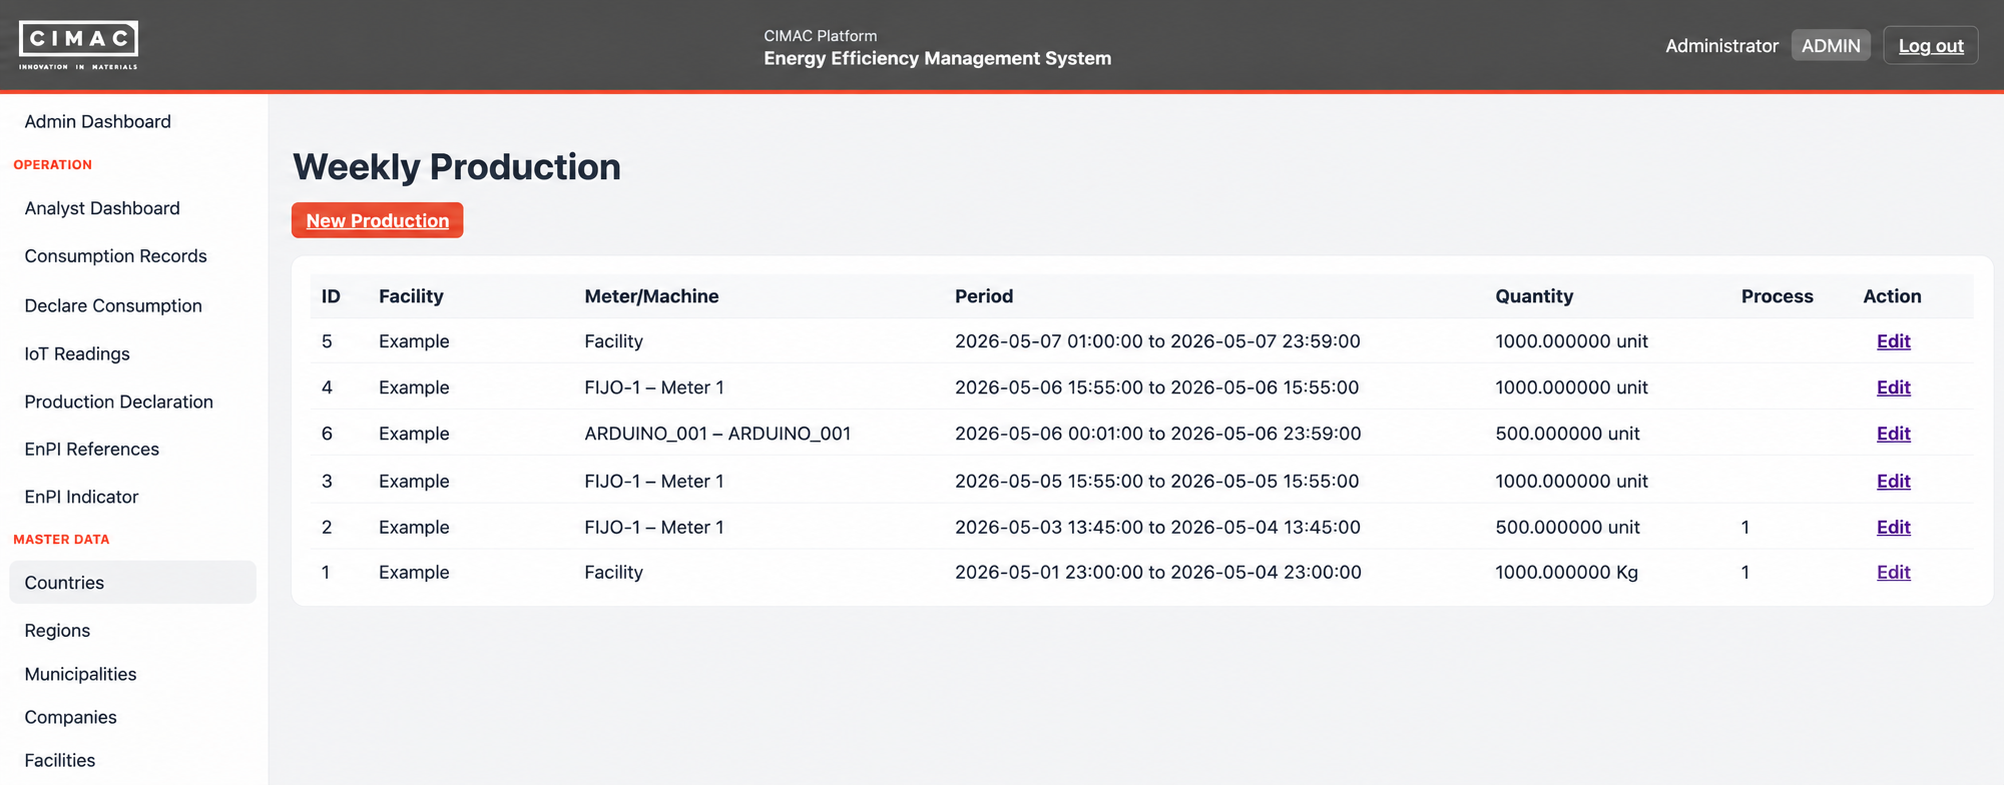
\includegraphics[width=0.90\textwidth]{figures/image4.png}
\caption{Supplementary weekly production module used to relate consumed energy to production quantity by facility, machine, or period.}
\label{fig:S2}
\end{figure}

\begin{figure}[H]
\centering

\includegraphics[width=0.55\textwidth]{adhesivo_enpi.png}
\caption{Supplementary physical installation sheet for the EnPi plug-and-play node. The displayed registration and credential fields correspond to a disabled demonstration view prepared for publication.}
\label{fig:S3}
\end{figure}

\begin{figure}[H]
\centering
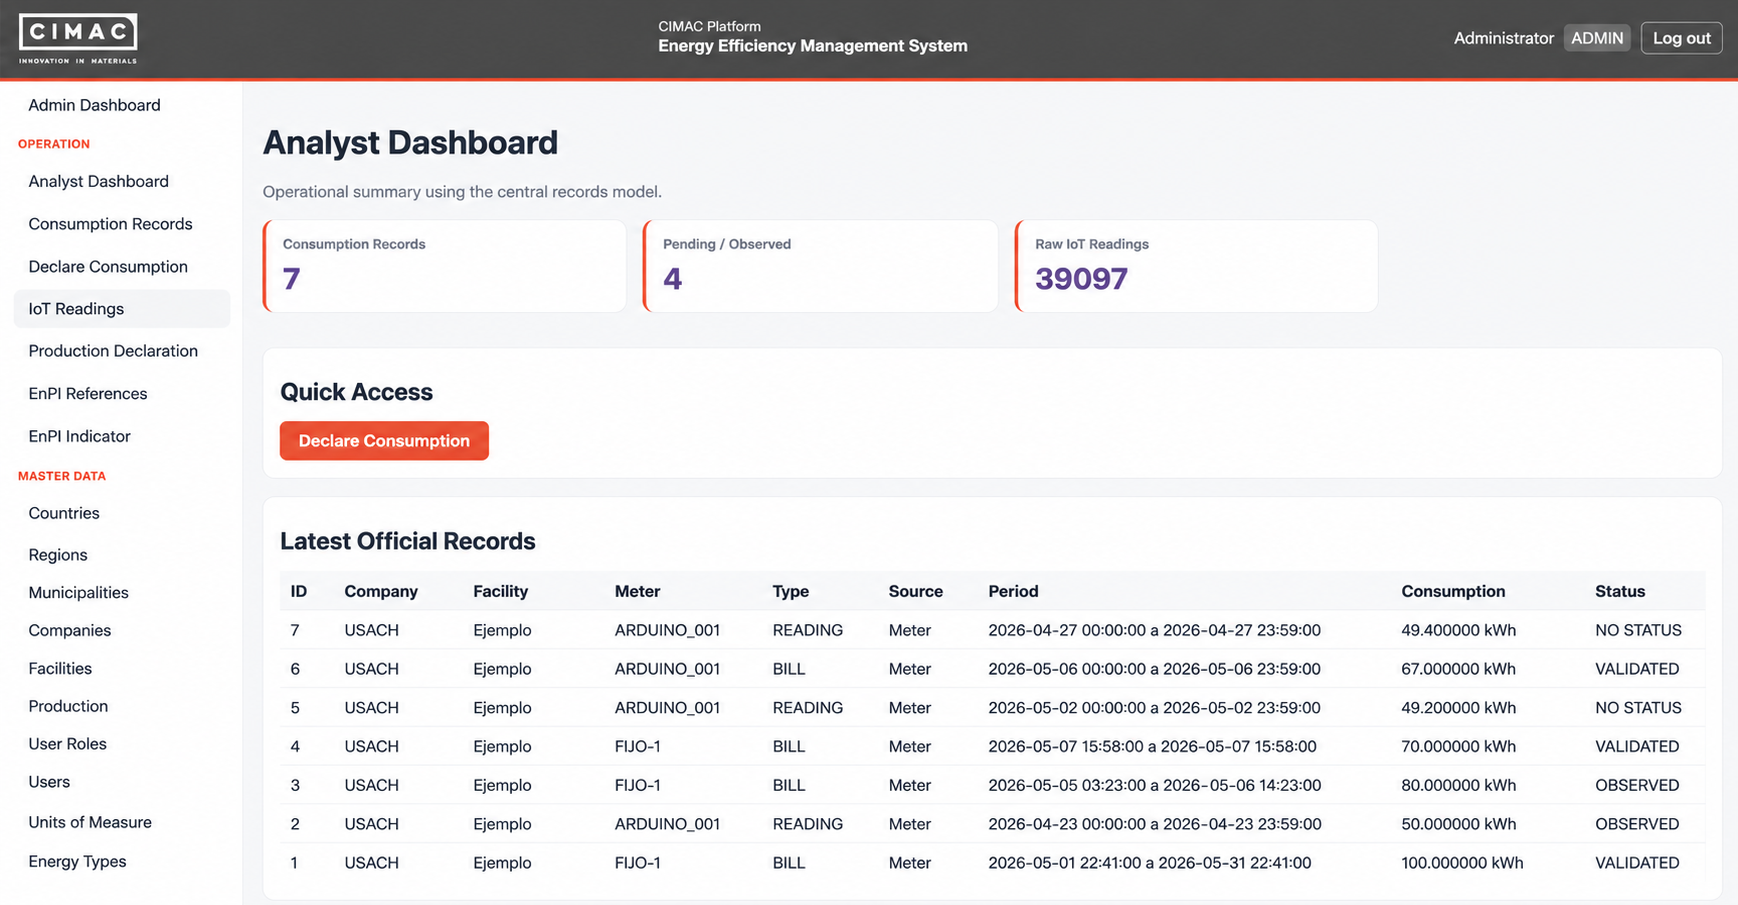
\includegraphics[width=0.90\textwidth]{figures/image6.png}
\caption{Supplementary operational dashboard with consumption records, raw IoT readings, and energy-data validation status.}
\label{fig:S4}
\end{figure}


\FloatBarrier

\section{Supplementary Reproducibility and Characterization Details}
\begin{table}[H]
\caption{Supplementary reproducibility information for the EnPi node and experimental pairing.}
\label{tab:S3}
\centering
\scriptsize
\begin{adjustbox}{max width=\textwidth}
\begin{tabular}{p{0.20\textwidth}p{0.36\textwidth}p{0.36\textwidth}}
\toprule
Element & Study implementation & Reproducibility and provenance note \\
\midrule
Node hardware & ESP32S3 as the transmission unit and PZEM-004T TTL Modbus-RTU single-phase 100 A module, interfaced via \texttt{PZEM004Tv30}. Rated range as per the commercial datasheet: 80--260 VAC, 0--100 A, 45--65 Hz, and power factor 0--1. The module was enclosed in a plug-and-play adapter with internal terminals and a male/female connector; the live wire supplying the dough sheeter runs in the internal metering point.  & The hardware configuration, acquisition module, and nominal operating ranges are reported to delimit the validated single-phase use case. \\
Firmware and sampling & The competing campaign utilized an ESP32S3 firmware branch with NTP time synchronization and direct delivery via HTTPS to the ingest endpoint. The exported trial logs for temporal coupling are at roughly one-second timestamp intervals. Features in the firmware branch 1.4.0 added during the campaign: assisted provisioning, remote configuration, RAM buffering, circular flash queue based on LittleFS, retransmission in chronological order after reconnecting to the internet, and OTA update capability. & The firmware used for the reported characterization and the subsequent operational-continuity branch are distinguished. The buffering and OTA improvements were not used to retrospectively modify the validation dataset. \\
Payload and transformation & \texttt{payload\_raw} corresponds to the raw reading transmitted by the ESP32S3; no intermediate backend transformation exists before storage. & Raw payload field retained as auditable evidence; subsequent corrections are documented. \\
Temporal pairing & EnPi and Metrel records aligned by scenario/timestamp (rounded to the nearest second). One continuity check showed gaps for 15 rows (210 missing EnPi timestamps: 20 seconds in scenario 000, 10 in 002, 20 in 007, and 160 in 009). & Position has not been included in the pointwise metrics (missing values not interpolated). We used only observations that shared timestamps and summed cumulative energy. We treated any gaps as the end of a continuous section. For each section, we measured changes to the EnPi register and then summed those changes over all sections. You can download the pairing and continuity-audit files. \\
Metrel MI2883 & Power quality analyzer used as the operational reference, calibrated and certified by the Centro de Instrumentaci\'on y Desarrollo Electr\'onico (CIDE), Universidad de Santiago de Chile, under certificate CCE:814-2025 dated 20 October 2025; simultaneous measurement on the same circuit/phase conductor. & The calibration organization, certificate identifier, date, and simultaneous connection support traceability of the comparison. \\
Data and analysis files & The raw and processed datasets, synchronized observations, scenario-level metrics, and analysis files supporting the reported results are publicly available in the EnPi repository at \url{https://github.com/The-Terial/Enpi}. & The repository contains the folders and files needed to replicate the EnPi--Metrel comparison, operational case, communication-loss handling, tables, and figures. \\
\bottomrule
\end{tabular}
\end{adjustbox}
\end{table}
\FloatBarrier

\begin{table}[H]
\caption{Supplementary bill of materials for the designed EnPi PCB. The full editable BOM file is kept in the Reproducibility repository; this table includes the built components relevant to hardware traceability.}
\label{tab:S4}
\centering
\scriptsize
\begin{adjustbox}{max width=\textwidth}
\begin{tabular}{p{0.16\textwidth}p{0.48\textwidth}p{0.16\textwidth}p{0.15\textwidth}}
\toprule
Designator & Component/comment & Part number & Assembly type \\
\midrule
C1 & YAGEO CC0603KRX7R9BB104 & C14663 & SMT \\
C4 & YAGEO CC0603KRX7R9BB104 & C14663 & SMT \\
R1 & YAGEO RC0603JR-075K1L & C14677 & SMT \\
R2 & YAGEO RC0603JR-075K1L & C14677 & SMT \\
R5 & UNI-ROYAL 0603WAJ0103T5E & C15401 & SMT \\
R6 & UNI-ROYAL 0603WAJ0103T5E & C15401 & SMT \\
R8 & UNI-ROYAL 0603WAJ0103T5E & C15401 & SMT \\
C2 & Samsung Electro-Mechanics CL21A106KAYNNNE & C15850 & SMT \\
C3 & Samsung Electro-Mechanics CL21A106KAYNNNE & C15850 & SMT \\
J1 & Korean Hroparts Elec TYPE-C-31-M-12 & C165948 & SMT \\
U2 & HI-LINK HLK-PM01 & C209903 & Wave soldering \\
JP\_TERM1 & UNI-ROYAL 0603WAF0000T5E & C21189 & SMT \\
R\_TERM1 & UNI-ROYAL 0603WAF1200T5E & C22787 & SMT \\
R3 & UNI-ROYAL 0603WAF330JT5E & C23140 & SMT \\
R4 & UNI-ROYAL 0603WAF330JT5E & C23140 & SMT \\
U3 & TECH PUBLIC AP2112K-3.3TRG1 & C23380830 & SMT \\
J2 & BOOMELE 2.54 mm 1x4 female connector & C2718488 & Wave soldering \\
U4 & ESPRESSIF ESP32-S3-WROOM-1-N16 & C2913199 & SMT \\
F1 holder & Xucheng Elec 5$\times$20 mm fuse holder XC-7 & C3131 & Wave soldering \\
F1 fuse & SCHURTER 5$\times$20 mm time-lag fuse, T1A, 250 V AC & T1A 250 V & Replaceable cartridge \\
RESET1 & XKB Connection TS-1187A-B-A-B & C318884 & SMT \\
BOOT1 & XKB Connection TS-1187A-B-A-B & C318884 & SMT \\
J5 & DORABO DB2ER-5.08-3P-GN & C395739 & Wave soldering \\
R7 & UNI-ROYAL 0603WAF2002T5E & C4184 & SMT \\
J4 & Cixi Kefa Elec KF135T-10.16-3P & C475109 & Wave soldering \\
J3 & Cixi Kefa Elec KF135T-10.16-3P & C475109 & Wave soldering \\
U1 & TECH PUBLIC MAX3485ESA & C7603385 & SMT \\
\bottomrule
\end{tabular}
\end{adjustbox}
\end{table}
\FloatBarrier

\subsection{Segment-Preserving Bootstrap Reproducibility}

The bootstrap sensitivity analysis employed the 9,119 valid loaded observations that were included in the pooled direct active-power comparison. We applied a fixed-length circular moving-block bootstrap independently to each contiguous, valid scenario segment to preserve scenario and communication-gap boundaries. Each segment was resampled to its original length, and subsequent segment-level contributions were aggregated to produce the pooled MAE, RMSE, bias, and WMAPE. To perform their work, we used 2000 replicates per block length $L\in \{15,30,60,120\}$ and NumPy \texttt{default\_rng} seed $20261013+L$. This procedure captures the random error inherent in the problem due to the insufficient number of scenarios over which it is defined (cf. \cite{r2_kunsch,r2_politis,r2_gum}); it is not an estimate of device-to-device variability or a metrological uncertainty budget. 

\begin{table}[H]
\caption{Supplementary segment-preserving bootstrap results for pooled direct active-power metrics. The primary analysis uses $L=60$ observations. Sensitivity ranges report the smallest lower endpoint and the largest upper endpoint observed across $L=15$, 30, 60, and 120; they are not additional confidence intervals.}
\label{tab:S5}
\centering
\scriptsize
\begin{adjustbox}{max width=0.96\textwidth}
\begin{tabular}{lccc}
\toprule
Metric & Observed pooled estimate & 95\% percentile interval ($L=60$) & Endpoint sensitivity across all $L$ \\
\midrule
MAE (W) & 11.408 & 11.054--11.959 & 11.054--12.014 \\
RMSE (W) & 23.184 & 15.926--32.697 & 15.916--33.253 \\
Bias (W) & $-11.034$ & $-11.207$ to $-10.822$ & $-11.245$ to $-10.771$ \\
WMAPE (\%) & 1.773 & 1.718--1.854 & 1.718--1.869 \\
\bottomrule
\end{tabular}
\end{adjustbox}
\end{table}

The comparatively wide RMSE interval indicates the impact of occasional large-error observations. The small shift of the MAE, bias and WMAPE endpoints between block-length choices shows that the principal pooled inference is not based on a single assumed dependence scale. The executable analysis built in each of these papers is provided in the EnPi repository, along with the input data for all analyses, which is validated in the EnPi repository at \url{https://github.com/The-Terial/Enpi}.
\FloatBarrier

\begin{figure}[H]
\centering
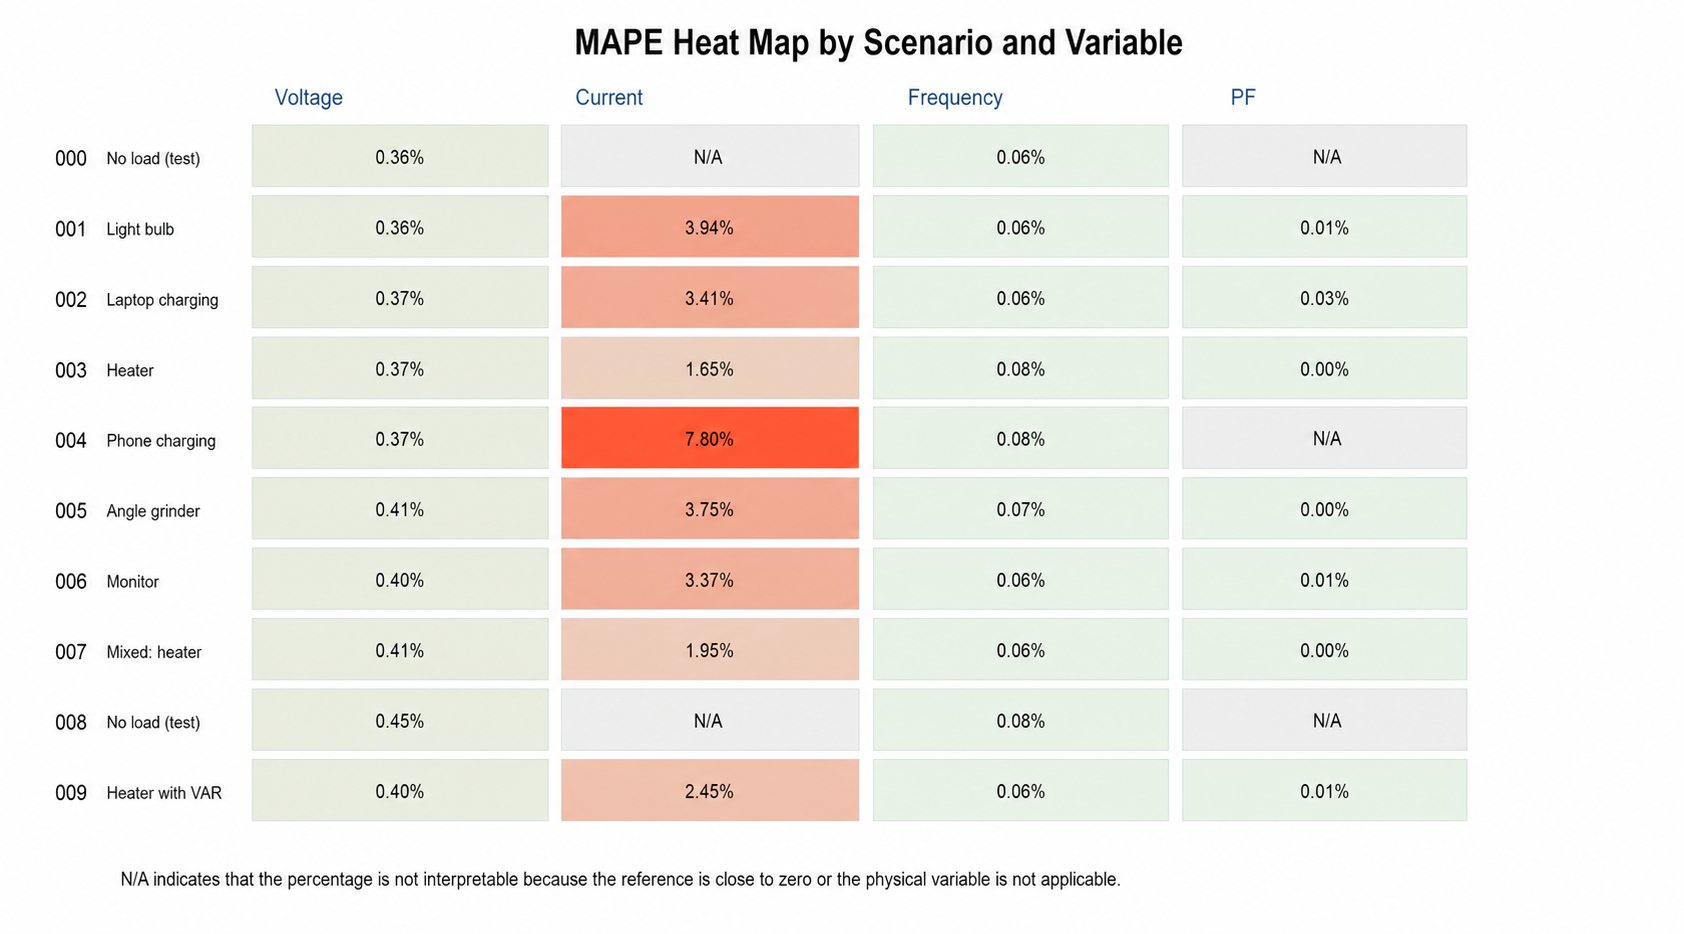
\includegraphics[width=0.88\textwidth]{figures/image8.png}
\caption{Supplementary MAPE heat map by scenario and variable.}
\label{fig:S5}
\end{figure}

\begin{figure}[H]
\centering
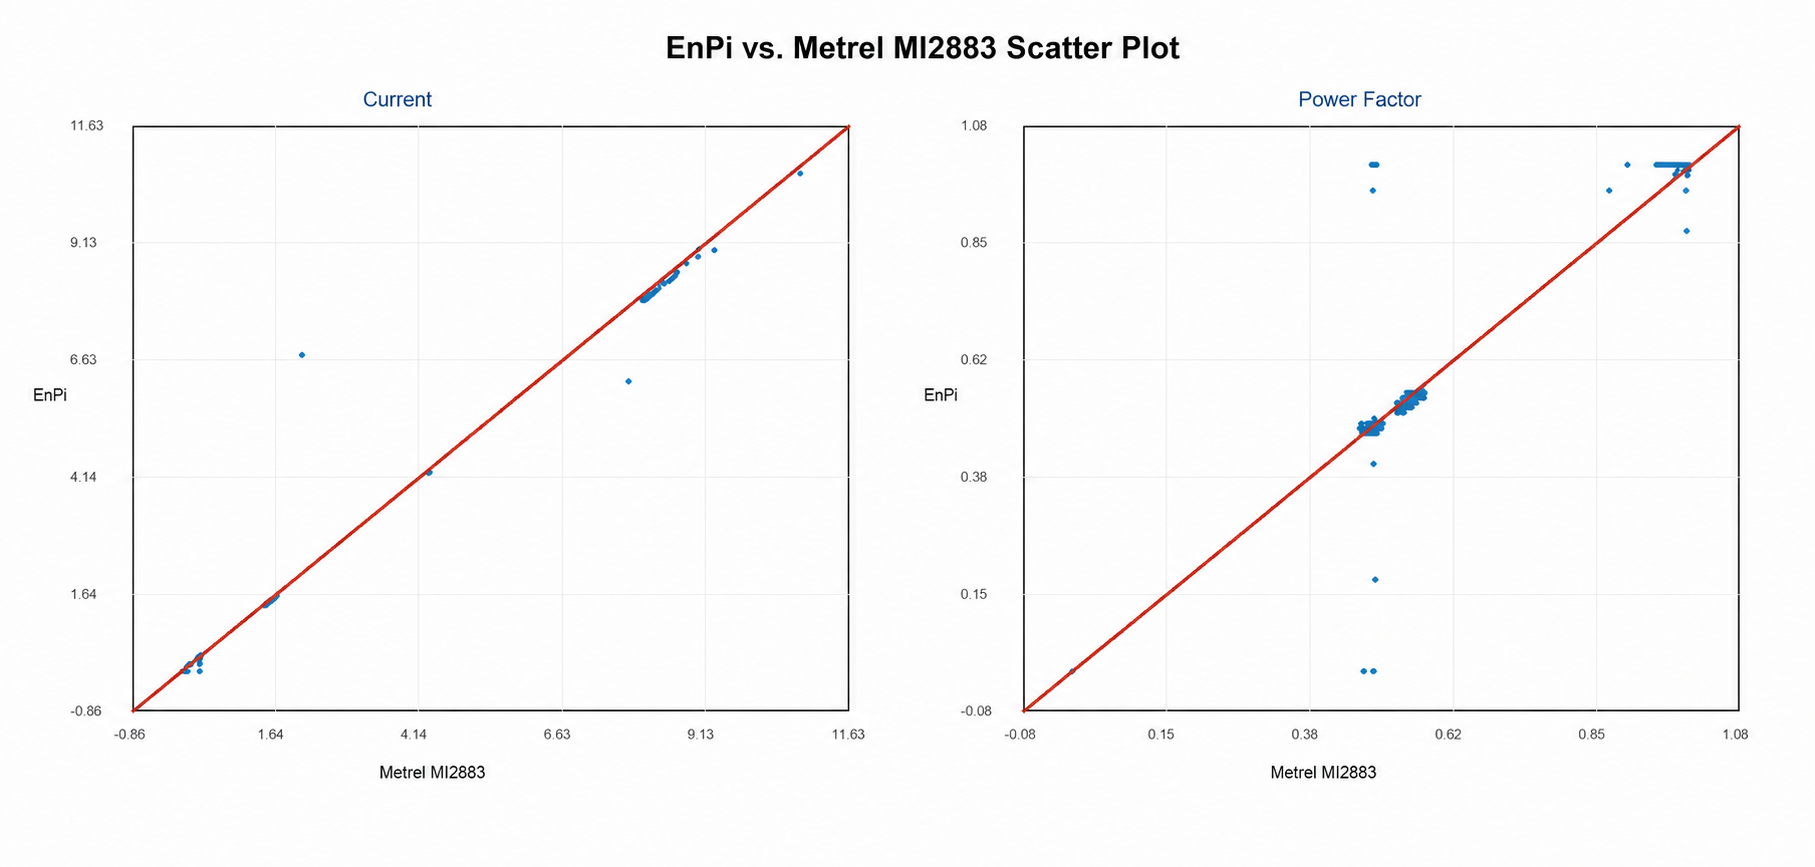
\includegraphics[width=0.88\textwidth]{figures/image9.png}
\caption{Supplementary EnPi--Metrel scatter plot for current and power factor. The red line represents ideal agreement, y=x.}
\label{fig:S6}
\end{figure}

\FloatBarrier

\section{Supplementary Firmware Continuity Logic}

The firmware source code, with credentials removed, is available in the public repository. The inspected post-campaign firmware branch implements an operational-continuity mechanism for intermittent connectivity. The mechanism was not used to correct or alter the EnPi--Metrel validation dataset; it documents the engineering response to the packet-loss limitation observed during the comparative campaign.

\subsection*{Supplementary Algorithm S1. Local buffering and chronological retransmission of non-transmitted readings}
\begin{enumerate}
\item Acquire voltage, current, active power, accumulated energy, frequency, and power factor from the PZEM interface.
\item Attach the original measurement timestamp, measurement duration, and configured acquisition interval to the reading.
\item Attempt direct HTTPS transmission to the ingestion endpoint.
\item If the transmission succeeds with an HTTP 2xx response, do not store a local copy.
\item If WiFi is unavailable, remote sending is disabled, the HTTP request fails, or the server rejects the request, append the reading to the RAM pending queue.
\item Periodically checkpoint RAM pending readings into a LittleFS circular flash queue to reduce flash wear during short interruptions.
\item If the flash queue reaches the configured capacity, overwrite the oldest pending reading first.
\item When WiFi connectivity is restored and remains stable, retransmit pending readings in chronological order: flash queue first, then RAM queue.
\item Remove a pending record only after successful server acknowledgement.
\item Before OTA update or remote restart, flush RAM pending readings to flash when buffering is enabled.
\end{enumerate}

\begin{figure}[H]
\centering
\begin{adjustbox}{max width=0.98\textwidth}
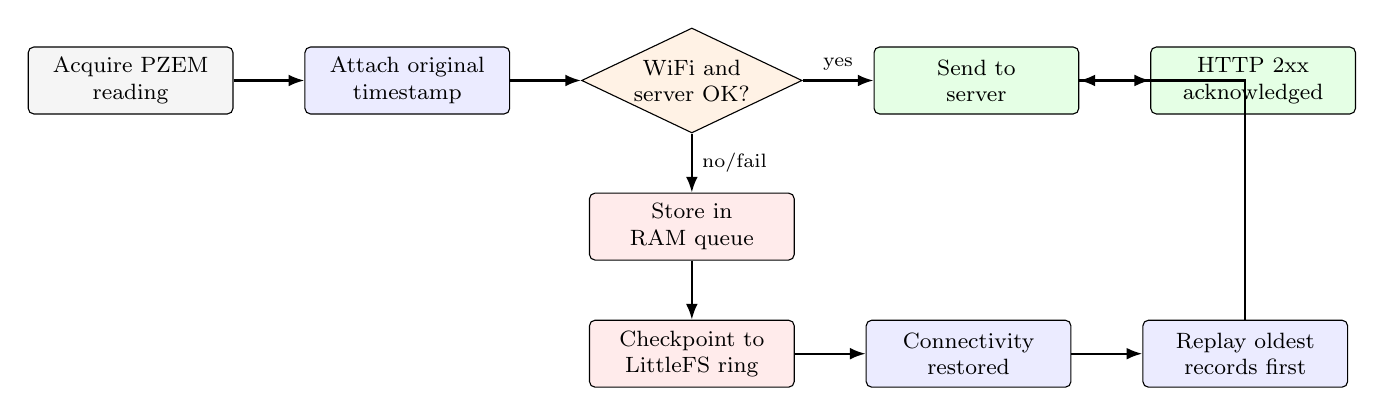
\begin{tikzpicture}[
    node distance=0.75cm and 0.9cm,
    block/.style={draw, rounded corners=2pt, align=center, minimum height=0.85cm, minimum width=2.6cm, font=\footnotesize},
    decision/.style={draw, diamond, aspect=2.1, align=center, inner sep=1pt, font=\footnotesize},
    arrow/.style={-{Latex[length=2mm]}, thick}
]
\node[block, fill=gray!8] (measure) {Acquire PZEM\\reading};
\node[block, fill=blue!8, right=of measure] (stamp) {Attach original\\timestamp};
\node[decision, fill=orange!10, right=of stamp] (wifi) {WiFi and\\server OK?};
\node[block, fill=green!10, right=of wifi] (send) {Send to\\server};
\node[block, fill=green!10, right=of send] (ack) {HTTP 2xx\\acknowledged};
\node[block, fill=red!8, below=of wifi] (ram) {Store in\\RAM queue};
\node[block, fill=red!8, below=of ram] (flash) {Checkpoint to\\LittleFS ring};
\node[block, fill=blue!8, right=of flash] (recover) {Connectivity\\restored};
\node[block, fill=blue!8, right=of recover] (replay) {Replay oldest\\records first};

\draw[arrow] (measure) -- (stamp);
\draw[arrow] (stamp) -- (wifi);
\draw[arrow] (wifi) -- node[above, font=\scriptsize] {yes} (send);
\draw[arrow] (send) -- (ack);
\draw[arrow] (wifi) -- node[right, font=\scriptsize] {no/fail} (ram);
\draw[arrow] (ram) -- (flash);
\draw[arrow] (flash) -- (recover);
\draw[arrow] (recover) -- (replay);
\draw[arrow] (replay) |- (send);
\end{tikzpicture}
\end{adjustbox}
\caption{Supplementary firmware continuity logic implemented after the comparative campaign. Non-transmitted readings are buffered locally with their original measurement timestamp and retransmitted chronologically after connectivity recovery. Records are deleted from the pending queue only after successful server acknowledgement.}
\label{fig:S7}
\end{figure}

\newpage
\section*{References}
\begin{thebibliography}{99}
\bibitem{ref1} M. U. Saleem, M. R. Usman, and M. Shakir, "Design, Implementation, and Deployment of an IoT Based Smart Energy Management System," IEEE Access, vol. 9, pp. 59649-59664, 2021, doi: 10.1109/ACCESS.2021.3070960.
\bibitem{ref2} M. Ullah, A. Narayanan, A. Wolff, and P. H. J. Nardelli, "Industrial Energy Management System: Design of a Conceptual Framework Using IoT and Big Data," IEEE Access, vol. 10, pp. 110557--110567, 2022, doi: 10.1109/ACCESS.2022.3215167.
\bibitem{ref3} Y. Li, Z. Sun, L. Han, and N. Mei, "Fuzzy Comprehensive Evaluation Method for Energy Management Systems Based on an Internet of Things," IEEE Access, vol. 5, pp. 21312-21322, 2017, doi: 10.1109/ACCESS.2017.2728081.
\bibitem{ref4} M. U. Saleem, M. R. Usman, M. A. Yaqub, A. Liotta, and A. Asim, "Smarter Grid in the 5G Era: Integrating the Internet of Things With a Cyber-Physical System," IEEE Access, vol. 12, pp. 34002--34018, 2024, doi: 10.1109/ACCESS.2024.3372379.
\bibitem{ref5} S. Kim, S. Lee, M. Kim, and Y. Kwon, "A Web Application Framework for Battery Health Prediction in Industrial IoT Networks," Journal of Web Engineering, vol. 24, no. 6, pp. 943-972, 2025, doi: 10.13052/jwe1540-9589.2464.
\bibitem{ref6} S. M. A. A. Abir, A. Anwar, J. Choi, and A. S. M. Kayes, "IoT-Enabled Smart Energy Grid: Applications and Challenges," IEEE Access, vol. 9, pp. 50961-50981, 2021, doi: 10.1109/ACCESS.2021.3067331.
\bibitem{ref7} Y. Santo, A. Abelem, A. Riker, and E. E. Tsiropoulou, "Integrating Data Privacy and Energy Management in Smart Cities With Partial Sustainable IoT Networks," IEEE Access, vol. 13, pp. 33176--33188, 2025, doi: 10.1109/ACCESS.2025.3541213.
\bibitem{ref8} O. Said, Z. Al-Makhadmeh, and A. Tolba, "EMS: An Energy Management Scheme for Green IoT Environments," IEEE Access, vol. 8, pp. 44983-44998, 2020, doi: 10.1109/ACCESS.2020.2976641.
\bibitem{ref9} B. Safaei, M. Peiravian, and M. Siamaki, "Eco-Friendly IoT: Leveraging Energy Harvesting for a Sustainable Future," IEEE Sensors Reviews, vol. 2, pp. 32--75, 2025, doi: 10.1109/SR.2025.3552043.
\bibitem{ref10} L. N. H. Pham, A. Shrestha, C. Sharma, and F. Gonzalez-Longatt, "Digital Twins and Cyber-Physical Systems Toward the Digitalization of Power and Energy Systems," IEEE Transactions on Technology and Society, vol. 6, no. 4, pp. 393--410, 2025, doi: 10.1109/TTS.2025.3615624.
\bibitem{ref11} M. S. Ahmad, N. N. Mansor, H. Mokhlis, K. Naidu, H. Mohamad, and F. Ramadhani, "Demand Response Program Toward Sustainable Power Supply: Current Status, Challenges, and Prospects in Malaysia," IEEE Access, vol. 13, pp. 34706--34731, 2025, doi: 10.1109/ACCESS.2025.3541841.
\bibitem{ref12} K. Shafique, B. A. Khawaja, F. Sabir, S. Qazi, and M. Mustaqim, "Internet of Things (IoT) for Next-Generation Smart Systems: A Review of Current Challenges, Future Trends and Prospects for Emerging 5G-IoT Scenarios," IEEE Access, vol. 8, pp. 23022-23040, 2020, doi: 10.1109/ACCESS.2020.2970118.
\bibitem{ref13} J. S. Yalli, M. H. Hasan, and A. A. Badawi, "Internet of Things (IoT): Origins, Embedded Technologies, Smart Applications, and Its Growth in the Last Decade," IEEE Access, vol. 12, pp. 91357--91382, 2024, doi: 10.1109/ACCESS.2024.3418995.
\bibitem{ref14} M. Soula, B. Mbarek, and A. Meddeb, "A Real-Time Trust Management Model Using Digital Twin in IoT Networks," IEEE Access, vol. 12, pp. 183326--183343, 2024, doi: 10.1109/ACCESS.2024.3506870.
\bibitem{ref15} A. Bounceur et al., "Phygital Twin IoT: A Hardware-Software Decomposition Architecture for Scalable and Secure Digital Twin IoT Systems," IEEE Open Journal of the Computer Society, vol. 7, pp. 755--768, 2026, doi: 10.1109/OJCS.2026.3681725.
\bibitem{ref16} A. Velez-Estevez, L. Gutierrez-Madronal, and I. Medina-Bulo, "IoT-TEG 4.0: A New Approach 4.0 for Test Event Generation," IEEE Transactions on Reliability, vol. 71, no. 3, pp. 1368--1380, 2022, doi: 10.1109/TR.2021.3087781.
\bibitem{ref17} M. S. Yaraziz and R. Hill, "Federated Q-Learning-Based Optimization for Resource Allocation in Industrial IoT Networks," IEEE Access, vol. 13, pp. 188880--188891, 2025, doi: 10.1109/ACCESS.2025.3624919.
\bibitem{ref18} H. Zhu, K. Ouahada, and A. M. Abu-Mahfouz, "Peer-to-Peer Energy Trading in Smart Energy Communities: A Lyapunov-Based Energy Control and Trading System," IEEE Access, vol. 10, pp. 42916--42932, 2022, doi: 10.1109/ACCESS.2022.3167828.
\bibitem{ref19} International Organization for Standardization, ISO 50001:2018, Energy management systems --- Requirements with guidance for use, Geneva, Switzerland: ISO, 2018.
\bibitem{ref20} International Organization for Standardization, ISO 50006:2023, Energy management systems --- Evaluating energy performance using energy performance indicators and energy baselines, Geneva, Switzerland: ISO, 2023.
\bibitem{ref21} G. W. Hart, ``Nonintrusive Appliance Load Monitoring,'' Proceedings of the IEEE, vol. 80, no. 12, pp. 1870--1891, Dec. 1992, doi: 10.1109/5.192069.
\bibitem{ref22} M. Briceño-León, D. Pazmiño-Quishpe, J.-M. Clairand, and G. Escrivá-Escrivá, ``Energy Efficiency Measures in Bakeries toward Competitiveness and Sustainability--Case Studies in Quito, Ecuador,'' Sustainability, vol. 13, no. 9, Art. no. 5209, 2021, doi: 10.3390/su13095209.
\bibitem{ref23} F. Paschino and F. Gambella, ``Comparison between traditional and industrial plants used for production of `carasau' bread and evaluation of final products,'' Applied Engineering in Agriculture, vol. 23, no. 1, pp. 65--70, 2007, doi: 10.13031/2013.22319.
\bibitem{ref24} J. Varela-Aldás, S. Silva, and G. Palacios-Navarro, ``IoT-Based Alternating Current Electrical Parameters Monitoring System,'' Energies, vol. 15, no. 18, Art. no. 6637, 2022, doi: 10.3390/en15186637.
\bibitem{ref25} International Electrotechnical Commission, IEC 62053-21:2020, Electricity metering equipment --- Particular requirements --- Part 21: Static meters for AC active energy (classes 0,5, 1 and 2), Geneva, Switzerland: IEC, 2020.
\bibitem{ref26} M. Jamshidi, ``System of Systems Engineering---New Challenges for the 21st Century,'' IEEE Aerospace and Electronic Systems Magazine, vol. 23, no. 5, pp. 4--19, May 2008, doi: 10.1109/MAES.2008.4523909.
\bibitem{ref27} D. Minoli, K. Sohraby, and B. Occhiogrosso, ``IoT Considerations, Requirements, and Architectures for Smart Buildings---Energy Optimization and Next-Generation Building Management Systems,'' IEEE Internet of Things Journal, vol. 4, no. 1, pp. 269--283, Feb. 2017, doi: 10.1109/JIOT.2017.2647881.
\bibitem{ref28} G. Bedi, G. K. Venayagamoorthy, R. Singh, R. R. Brooks, and K.-C. Wang, ``Review of Internet of Things (IoT) in Electric Power and Energy Systems,'' IEEE Internet of Things Journal, vol. 5, no. 2, pp. 847--870, Apr. 2018, doi: 10.1109/JIOT.2018.2802704.
\bibitem{r2_gum} Joint Committee for Guides in Metrology, \emph{Evaluation of Measurement Data---Guide to the Expression of Uncertainty in Measurement}, JCGM 100:2008, 2008, doi: 10.59161/JCGM100-2008E.
\bibitem{r2_vim} Joint Committee for Guides in Metrology, \emph{International Vocabulary of Metrology---Basic and General Concepts and Associated Terms}, JCGM 200:2012, 2012, doi: 10.59161/JCGM200-2012.
\bibitem{r2_iso50015} International Organization for Standardization, \emph{ISO 50015:2014---Energy Management Systems---Measurement and Verification of Energy Performance of Organizations---General Principles and Guidance}, 2014.
\bibitem{r2_kunsch} H. R. K\"unsch, ``The jackknife and the bootstrap for general stationary observations,'' \emph{Annals of Statistics}, vol. 17, no. 3, pp. 1217--1241, 1989, doi: 10.1214/aos/1176347265.
\bibitem{r2_politis} D. N. Politis and J. P. Romano, ``The stationary bootstrap,'' \emph{Journal of the American Statistical Association}, vol. 89, no. 428, pp. 1303--1313, 1994, doi: 10.1080/01621459.1994.10476870.
\bibitem{r2_ntp} D. Mills, J. Martin, J. Burbank, and W. Kasch, \emph{Network Time Protocol Version 4: Protocol and Algorithms Specification}, RFC 5905, 2010, doi: 10.17487/RFC5905.
\bibitem{r2_prov} T. Lebo, S. Sahoo, and D. McGuinness, \emph{PROV-O: The PROV Ontology}, W3C Recommendation, 2013.
\bibitem{r2_tls} E. Rescorla, \emph{The Transport Layer Security (TLS) Protocol Version 1.3}, RFC 8446, 2018, doi: 10.17487/RFC8446.
\bibitem{r2_bland} J. M. Bland and D. G. Altman, ``Statistical methods for assessing agreement between two methods of clinical measurement,'' \emph{The Lancet}, vol. 327, no. 8476, pp. 307--310, 1986, doi: 10.1016/S0140-6736(86)90837-8.
\bibitem{r2_hyndman} R. J. Hyndman and A. B. Koehler, ``Another look at measures of forecast accuracy,'' \emph{International Journal of Forecasting}, vol. 22, no. 4, pp. 679--688, 2006, doi: 10.1016/j.ijforecast.2006.03.001.
\bibitem{r2_rfc3339} G. Klyne and C. Newman, \emph{Date and Time on the Internet: Timestamps}, RFC 3339, 2002, doi: 10.17487/RFC3339.
\bibitem{r2_gubbi} J. Gubbi, R. Buyya, S. Marusic, and M. Palaniswami, ``Internet of Things (IoT): A vision, architectural elements, and future directions,'' \emph{Future Generation Computer Systems}, vol. 29, no. 7, pp. 1645--1660, 2013, doi: 10.1016/j.future.2013.01.010.
\bibitem{r2_shi} W. Shi, J. Cao, Q. Zhang, Y. Li, and L. Xu, ``Edge Computing: Vision and Challenges,'' \emph{IEEE Internet of Things Journal}, vol. 3, no. 5, pp. 637--646, 2016, doi: 10.1109/JIOT.2016.2579198.
\bibitem{r2_khasawneh2025} H. J. Khasawneh, R. Al Asbahi, A. W. Alzariqi, D. R. Al Qada, A. Bujuk, M. A. Nawfal, and M. Tareen, ``Industrial IoT-based submetering solution for real-time energy monitoring,'' \emph{Discover Internet of Things}, vol. 5, art. 15, 2025, doi: 10.1007/s43926-025-00110-y.
\bibitem{r2_mirani2024} A. A. Mirani, A. Awasthi, N. O'Mahony, and J. Walsh, ``Industrial IoT-Based Energy Monitoring System: Using Data Processing at Edge,'' \emph{IoT}, vol. 5, no. 4, pp. 608--633, 2024, doi: 10.3390/iot5040027.
\bibitem{r3_sousa2023} E. L. de Sousa, L. A. de Aquino Marques, I. da S. Felix de Lima, A. B. M. Neves, E. N. Cunha, M. E. Kreutz, and A. J. V. Neto, ``Development a Low-Cost Wireless Smart Meter with Power Quality Measurement for Smart Grid Applications'', \emph{Sensors}, vol. 23, no. 16, art. 7210, 2023, doi: 10.3390/s23167210.
\bibitem{r3_openz2018} E. Viciana, A. Alcayde, F. G. Montoya, R. Ba\~nos, F. M. Arrabal-Campos, A. Zapata-Sierra, and F. Manzano-Agugliaro, ``OpenZmeter: An Efficient Low-Cost Energy Smart Meter and Power Quality Analyzer,'' \emph{Sustainability}, vol. 10, no. 11, art. 4038, 2018, doi: 10.3390/su10114038.
\bibitem{r3_khan2024} H. R. Khan, M. Kazmi, Lubaba, M. H. Bin Khalid, U. Alam, K. Arshad, K. Assaleh, and S. A. Qazi, ``A Low-Cost Energy Monitoring System with Universal Compatibility and Real-Time Visualization for Enhanced Accessibility and Power Savings'', \emph{Sustainability}, vol. 16, no. 10, art. 4137, 2024, doi: 10.3390/su16104137.
\bibitem{r3_iotmeter2022} O. Munoz, A. Ruelas, P. Rosales, A. Acu\~na, A. Suastegui, and F. Lara, ``Design and Development of an IoT Smart Meter with Load Control for Home Energy Management Systems,'' \emph{Sensors}, vol. 22, no. 19, art. 7536, 2022, doi: 10.3390/s22197536.
\bibitem{r3_calibration2019} F. Sanchez-Sutil, A. Cano-Ortega, J. C. Hernandez, and C. Rus-Casas, ``Development and Calibration of an Open Source, Low-Cost Power Smart Meter Prototype for PV Household-Prosumers'', \emph{Electronics}, vol. 8, no. 8, art. 878, 2019, doi: 10.3390/electronics8080878.
\bibitem{r3_conti2023} G. Conti, D. Jimenez, A. del Rio, S. Castano-Solis, J. Serrano, and J. Fraile-Ardanuy, ``A Multi-Port Hardware Energy Meter System for Data Centers and Server Farms Monitoring'', \emph{Sensors}, vol. 23, no. 1, art. 119, 2023, doi: 10.3390/s23010119.
\bibitem{r3_iiot2022} R. Bin Mofidul, M. M. Alam, M. H. Rahman, and Y. M. Jang, ``Real-Time Energy Data Acquisition, Anomaly Detection, and Monitoring System: Implementation of a Secured, Robust, and Integrated Global IIoT Infrastructure with Edge and Cloud AI'', \emph{Sensors}, vol. 22, no. 22, art. 8980, 2022, doi: 10.3390/s22228980.
\bibitem{r3_hierarchy2020} B. Beisheim, S. Kr\"amer, and S. Engell, ``Hierarchical aggregation of energy performance indicators in continuous production processes,'' \emph{Applied Energy}, vol. 264, art. 114709, 2020, doi: 10.1016/j.apenergy.2020.114709.
\bibitem{r3_kraft2021} E. Andersson, H. Derneg\aa rd, M. Wall\'en, and P. Thollander, ``Decarbonization of industry: Implementation of energy performance indicators for successful energy management practices in kraft pulp mills'', \emph{Energy Reports}, vol. 7, pp. 1808--1817, 2021, doi: 10.1016/j.egyr.2021.03.009.
\bibitem{r3_piccioni2024} M. Piccioni, F. Martini, C. Martini, and C. Toro, ``Evaluation of Energy Performance Indicators and Energy Saving Opportunities for the Italian Rubber Manufacturing Industry'', \emph{Energies}, vol. 17, no. 7, art. 1584, 2024, doi: 10.3390/en17071584.
\bibitem{r3_korea2021} H.-S. Shim and S.-J. Lee, ``Investigating the Use of Energy Performance Indicators in Korean Industry Sector'', \emph{Journal of the Korea Academia-Industrial Cooperation Society}, vol. 22, no. 3, pp. 707--725, 2021, doi: 10.5762/KAIS.2021.22.3.707.
\bibitem{r3_rubber2020} F. M. Kanchiralla, N. Jalo, S. Johnsson, P. Thollander, and M. Andersson, ``Energy End-Use Categorization and Performance Indicators for Energy Management in the Engineering Industry'', \emph{Energies}, vol. 13, no. 2, art. 369, 2020, doi: 10.3390/en13020369.
\bibitem{r3_atenea2025} A. Ferraro, G. Bruni, M. Salvio, M. Marroccoli, A. Telesca, C. Martini, F. A. Tocchetti, and A. D'Angola, ``ATENEA4SME: Industrial SME Self-Evaluation of Energy Efficiency'', \emph{Energies}, vol. 18, no. 15, art. 4094, 2025, doi: 10.3390/en18154094.
\bibitem{r3_review2024} B. Ioshchikhes, M. Frank, and M. Weigold, ``A Systematic Review of Expert Systems for Improving Energy Efficiency in the Manufacturing Industry'', \emph{Energies}, vol. 17, no. 19, art. 4780, 2024, doi: 10.3390/en17194780.
\bibitem{r3_enpi2026} Y. Castillo Alvarez, R. Jim\'enez Borges, J. P. Monteagudo Yanes, A. Y. Resendiz Jaramillo, L. A. I. Carrera, H. Rodr\'iguez-Res\'endiz, and J. Rodr\'iguez-Res\'endiz, ``A Multistage Sufficiency Test for Selecting Energy Performance Indicators in Industry: Beyond $R^{2}$ Toward the Variable Associated with Significant Energy Use'', \emph{Processes}, vol. 14, no. 16, art. 2676, 2026, doi: 10.3390/pr14162676.
\end{thebibliography}

\end{document}
